% Options for packages loaded elsewhere
\PassOptionsToPackage{unicode}{hyperref}
\PassOptionsToPackage{hyphens}{url}
%
\documentclass[
]{article}
\usepackage{amsmath,amssymb}
\usepackage{lmodern}
\usepackage{iftex}
\ifPDFTeX
  \usepackage[T1]{fontenc}
  \usepackage[utf8]{inputenc}
  \usepackage{textcomp} % provide euro and other symbols
\else % if luatex or xetex
  \usepackage{unicode-math}
  \defaultfontfeatures{Scale=MatchLowercase}
  \defaultfontfeatures[\rmfamily]{Ligatures=TeX,Scale=1}
\fi
% Use upquote if available, for straight quotes in verbatim environments
\IfFileExists{upquote.sty}{\usepackage{upquote}}{}
\IfFileExists{microtype.sty}{% use microtype if available
  \usepackage[]{microtype}
  \UseMicrotypeSet[protrusion]{basicmath} % disable protrusion for tt fonts
}{}
\makeatletter
\@ifundefined{KOMAClassName}{% if non-KOMA class
  \IfFileExists{parskip.sty}{%
    \usepackage{parskip}
  }{% else
    \setlength{\parindent}{0pt}
    \setlength{\parskip}{6pt plus 2pt minus 1pt}}
}{% if KOMA class
  \KOMAoptions{parskip=half}}
\makeatother
\usepackage{xcolor}
\usepackage[margin=1in]{geometry}
\usepackage{graphicx}
\makeatletter
\def\maxwidth{\ifdim\Gin@nat@width>\linewidth\linewidth\else\Gin@nat@width\fi}
\def\maxheight{\ifdim\Gin@nat@height>\textheight\textheight\else\Gin@nat@height\fi}
\makeatother
% Scale images if necessary, so that they will not overflow the page
% margins by default, and it is still possible to overwrite the defaults
% using explicit options in \includegraphics[width, height, ...]{}
\setkeys{Gin}{width=\maxwidth,height=\maxheight,keepaspectratio}
% Set default figure placement to htbp
\makeatletter
\def\fps@figure{htbp}
\makeatother
\setlength{\emergencystretch}{3em} % prevent overfull lines
\providecommand{\tightlist}{%
  \setlength{\itemsep}{0pt}\setlength{\parskip}{0pt}}
\setcounter{secnumdepth}{-\maxdimen} % remove section numbering
\ifLuaTeX
  \usepackage{selnolig}  % disable illegal ligatures
\fi
\IfFileExists{bookmark.sty}{\usepackage{bookmark}}{\usepackage{hyperref}}
\IfFileExists{xurl.sty}{\usepackage{xurl}}{} % add URL line breaks if available
\urlstyle{same} % disable monospaced font for URLs
\hypersetup{
  pdftitle={Project 5 Gene interaction},
  pdfauthor={Melissa Kang and Seth Peacock},
  hidelinks,
  pdfcreator={LaTeX via pandoc}}

\title{Project 5 Gene interaction}
\author{Melissa Kang and Seth Peacock}
\date{2022-08-11}

\begin{document}
\maketitle

\hypertarget{introduction-and-problem-statement}{%
\subsection{Introduction and Problem
Statement}\label{introduction-and-problem-statement}}

Genes are fundamental to cell biology. Some gene may cause others to not
be express, repress, some may cause them to be expressed more, activate,
some may repress or activate themselves, or have no interaction with
other genes. Key genes determine cell development. Considering many
genes in a cell together, a (one-direction) network can model the
interactions between the genes, where an edge may indicate activation or
indicate repression. A large network of many genes is build up from
network motifs between pairs of genes. Knowing these motifs, then, can
inform modeling of large gene networks and and understanding cell
development. The network links, however, not so clear that they can be
observed directly. What can be observed is the number of gene A and gene
B across many cells. These provide counts which may be transformed to
estimate a bivariate probability mass function (pmf) for the two genes.
The bivariate pmf is, in part, the result of the underlying motif.
Predicting the motif based on the pmf may, therefore, be possible. The
To this end, we used supervised machine learning to predict the motif
given the pmf. This required that we know the underlining motif, so the
Read Lab estimated the pmfs for the motifs using simulation.

Prediction-modeling performance is pending.

\hypertarget{background-and-related-work}{%
\subsection{Background and related
work}\label{background-and-related-work}}

Describe relevant scientific background and point to work that tried to
solve similar problems in the past. Provide a few references to
textbooks and/or research articles that describe relevant background.

Stochastic models of gene regulatory networks have been tremendously
influential towards understanding cellular heterogeneity and analyzing
data from single-cell RNA sequencing (scRNA-seq). In order to further
understand single-cell gene pair interactions, stochastic models have
been used to produce gene-pair co-expression landscapes from a bivariate
distribution (Gallivan et al.~(2020)). Gallivan et al.~have developed a
family of stochastic gene-gene interaction models because existing
single-cell data analysis techniques have mostly disregarded that
pair-wise gene interactions can be deduced from the shapes of these
landscapes (2020). Shannon Entropy, Peason Correlation Coefficient,
Mutual Information, and a Coexpression Index were found to be relatively
inaccurate predictors of landscape shape of a gene-gene interaction on
their own, so the student researchers added mean and standard deviation
to the list of features to train the models (Gallivan et al.~(2020)).

In another relevant article, Cao, J., Spielmann, M., Qiu, X. et al.~have
used scRNA-seq on two million cells from mouse embryo in attempt to
obtain a more comprehensive view of the mouse oranogenesis cell atlas
(MOCA) and developmental processes (Cao, J., Spielmann, M., Qiu, X. et
al.~(2019)). The student researchers have used the data collected for
this experiment to visualize the gene-pair bivariate pmfs used for the
stochastic models and to test whether the models trained on the
simulated data can distinguish the motif of a landscape.

\hypertarget{data-and-exploratory-data-analysis}{%
\subsection{Data and exploratory data
analysis}\label{data-and-exploratory-data-analysis}}

Describe what data set(s) you used in the project -- include references
(e.g., URLs) for where you obtained the data if you can. This section
should have considerable detail -- make sure you include a good
description of your data set(s), including size, dimensionality, types
of variables, etc. Use figures (histograms, scatter plots, etc) and
tables, but do not overwhelm the reader with too many plots and show
only plots that provide interesting insights. In your writing, try to
give the reader some intuition and sense of what your data is like.

\hypertarget{experimental-data}{%
\subsubsection{Experimental Data}\label{experimental-data}}

The data was transformed into a h5 file from
\url{https://oncoscape.v3.sttrcancer.org/atlas.gs.washington.edu.mouse.rna/downloads}
gene\_count.txt.

The rows of the sparse matrix are cells, and the columns are genes. The
dataset is (11376, 26183), so there are 11376 cells and 26183 genes. The
dataset from the h5 file has been transformed into a sparse matrix, but
a sample of it is not shown here because it is mostly zeroes. Instead,
the histogram below shows the distribution of values in the sparse
matrix. The 2d plot was created from the entire sparse matrix and
reinforces the idea that some genes are more commonly expressed than
others. This is shown by the vertical striations seen in the graph for
genes that are expressed in many cells. Other genes are seen as
whitespace because they are hardly expressed at all.

\hypertarget{section}{%
\section{\texorpdfstring{\protect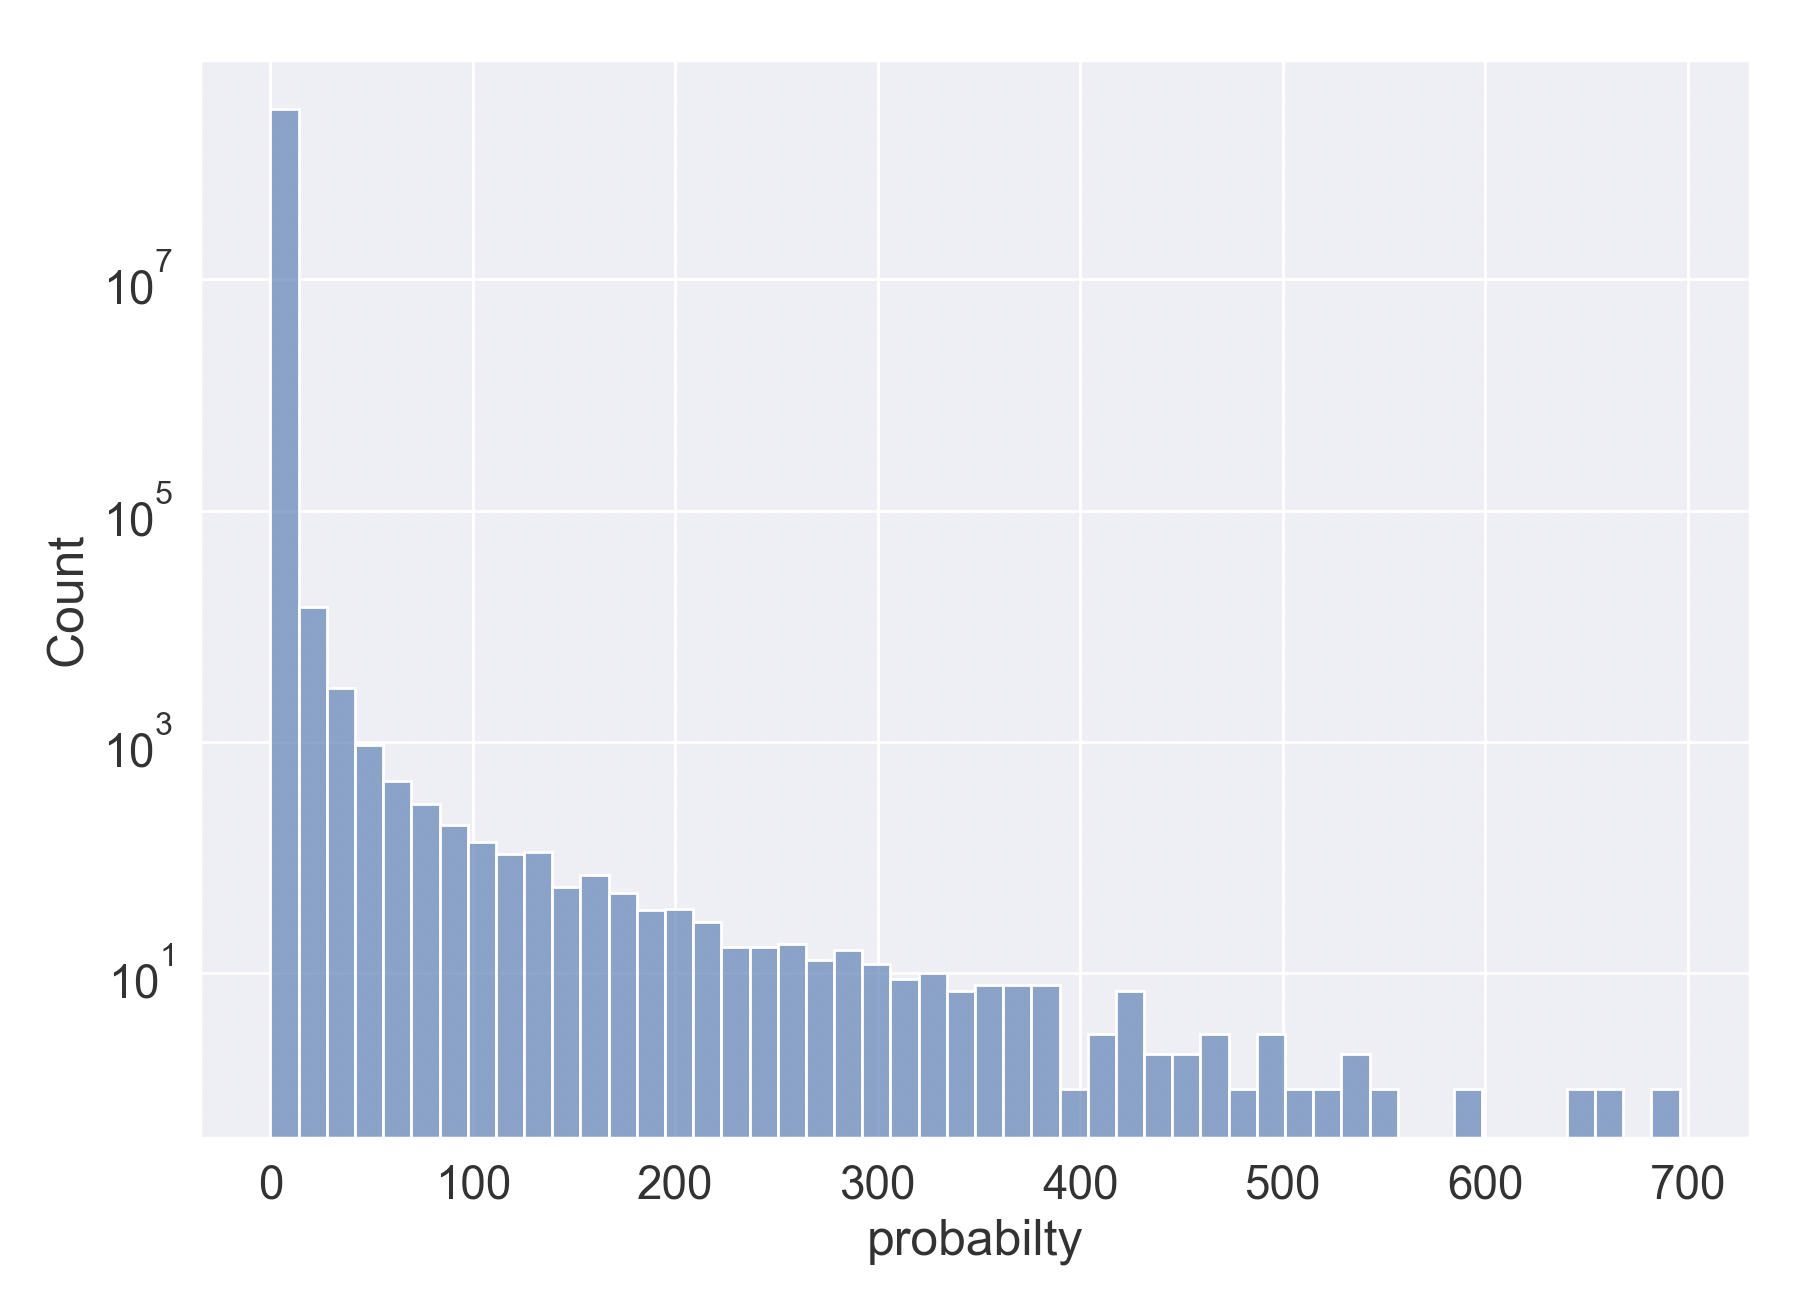
\includegraphics{../analysis/eda/h5-plots/gene_count.png}}{}}\label{section}}

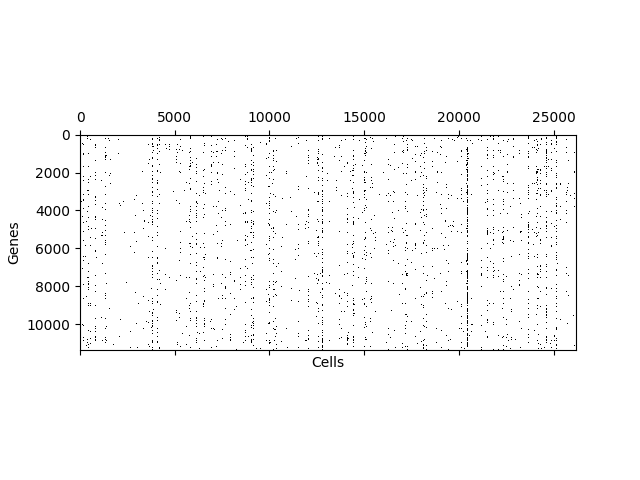
\includegraphics{../analysis/eda/h5-plots/2d-plot.png}

\begin{verbatim}
##        0      1      2      3      4      ...  11371  11372  11373  11374  11375
## 23560     14     10    197     11     53  ...     13     25     16     79     35
## 7942       0      0      1      2      7  ...      1      2      3      0      4
## 19548     16      0     25      3      1  ...      0      1      0      0     12
## 24692     15      2     11      0      0  ...      0      2      0     10     10
## 26165      1      7     20      0      6  ...      4     32     31     12     16
## 
## [5 rows x 11376 columns]
\end{verbatim}

The top\_26\_df is a Dataframe of the 26 most expressed genes in the
sparse matrix. There are 26 rows for the 26 genes and there are 11376
columns for the original amount of cells. This Dataframe was used to
create gene-gene interaction heatmap plots for each distinct interaction
between the 26 genes. The axis of the plots are the gene counts and the
coloring scale represents the number of cells with the combination of
gene counts. Below are two of the plots made.

From the afp vs meg3 plot, we can infer that cells that express a large
amount of Afp also tend to express a large amount of Meg3. Therefore, we
are expecting a motif identifier that expresses a fairly equal
relationship between the two genes. The meg3 vs gpc3 plot shows that
cells that express a large amount of Gpc3 tend to express a lower amount
of Meg3, so we expect a motif identifer that favors one of the genes
over the other.

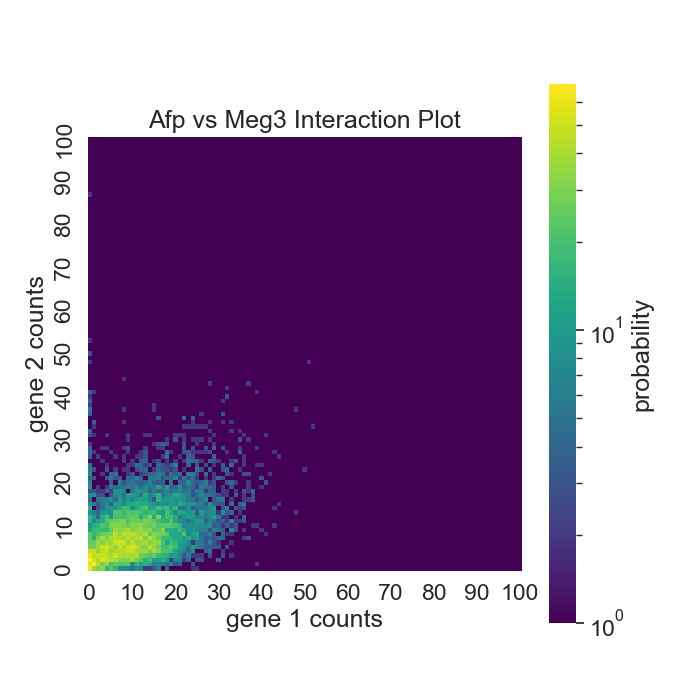
\includegraphics{../analysis/eda/h5-plots/Gene1-Afp-vs-Gene2-Meg3-hm.png}
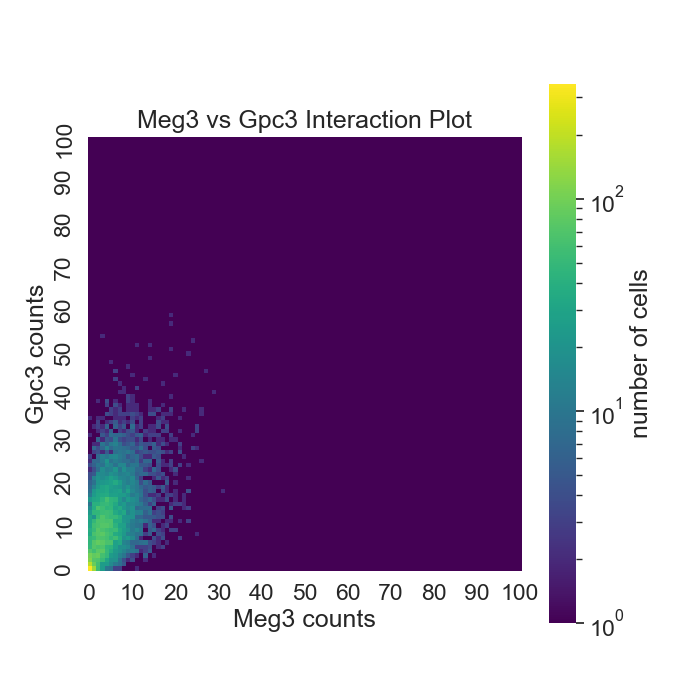
\includegraphics{../analysis/eda/h5-plots/Gene1-Meg3-vs-Gene2-Gpc3-hm.png}

\hypertarget{simulated-data}{%
\subsubsection{Simulated Data}\label{simulated-data}}

These data were generated by the Read Lab using the stochastic model
which Gallivan et al.~introduced (2019). We used multiple simulated data
sets. The first we received (hereafter ) had pmf estimates for all 81
gene pair motifs, approximately 60 replicates, each using different rate
parameters, per motif. The pmf's domain was two counts, starting at zero
and truncated at fifty. This pmf was vectorized (length 2601). Each of
the columns, then, has the estimated probability that a given cell would
have \(x_i\) gene X and \(y_i\) of Y for the rates specified for that
replicate. We added to each row the motif identifier, which is four
digits. The first digit identifies what gene X does to itself, the
second what gene X does to gene Y, the third what Y does to X, and the
fourth what Y does to itself. Each digit may be 1 for activation, 0 for
not interaction, or -1 for repression. Here is the first five rows of
the data frame.

\begin{verbatim}
##           id    p(0,0)    p(0,1)  ...  p(50,48)  p(50,49)  p(50,50)
## 0   0 0 -1 0  0.000404  0.001817  ...       0.0       0.0       0.0
## 1    0 0 0 0  0.049071  0.076737  ...       0.0       0.0       0.0
## 2   1 1 -1 1  0.000202  0.000606  ...       0.0       0.0       0.0
## 3  1 -1 1 -1  0.000000  0.000202  ...       0.0       0.0       0.0
## 4   1 1 1 -1  0.000000  0.000202  ...       0.0       0.0       0.0
## 
## [5 rows x 2602 columns]
\end{verbatim}

The vector of probabilities for a row may be transformed to a 51x51
matrix and visualized using a heat map. Here are some examples:

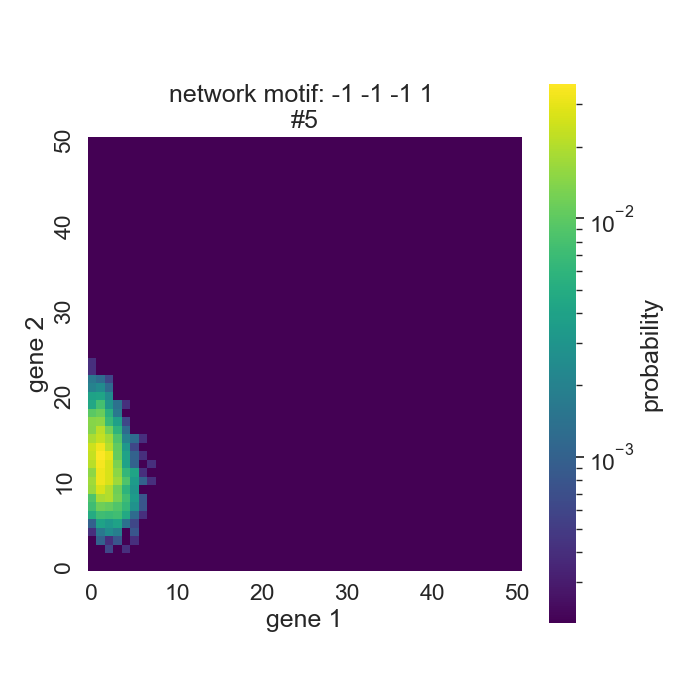
\includegraphics{../analysis/eda/first-set-heatmaps/sample/motif-03-i-05-row-4976.png}
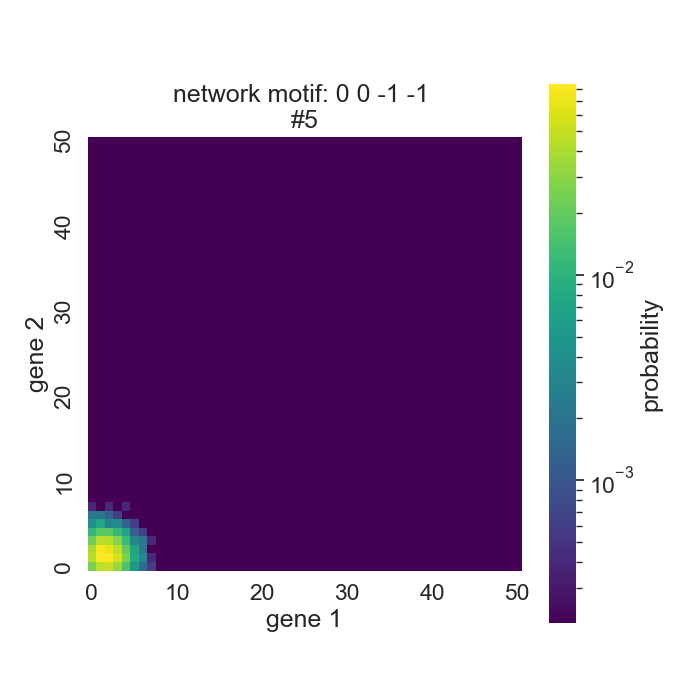
\includegraphics{../analysis/eda/first-set-heatmaps/sample/motif-37-i-05-row-1663.png}

The following are summary statistics of two motifs.
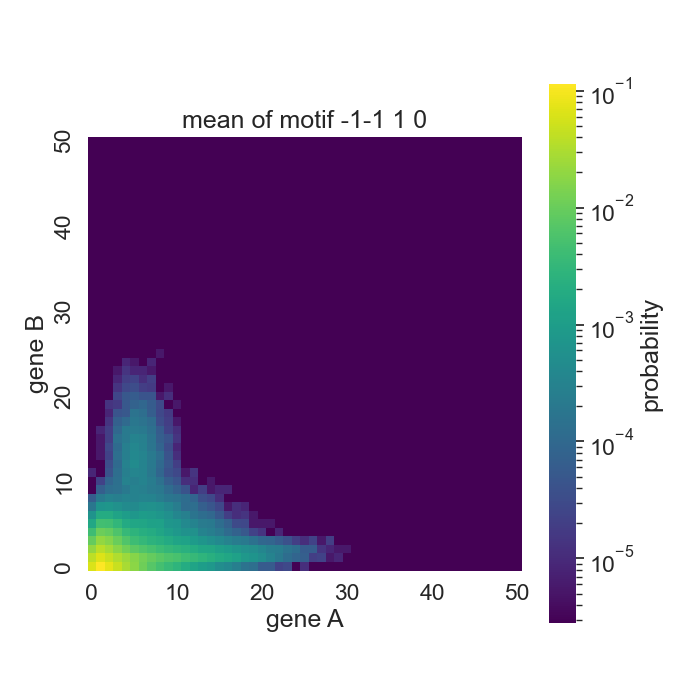
\includegraphics{../analysis/eda/first-set-heatmaps/summaries/08-mean.png}
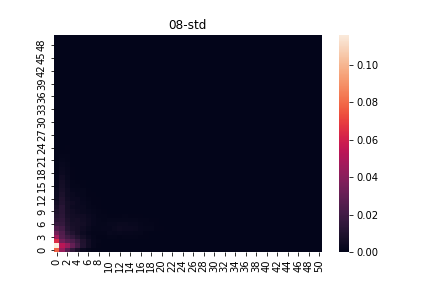
\includegraphics{../analysis/eda/first-set-heatmaps/summaries/08-std.png}

This motif varies quite a bit.

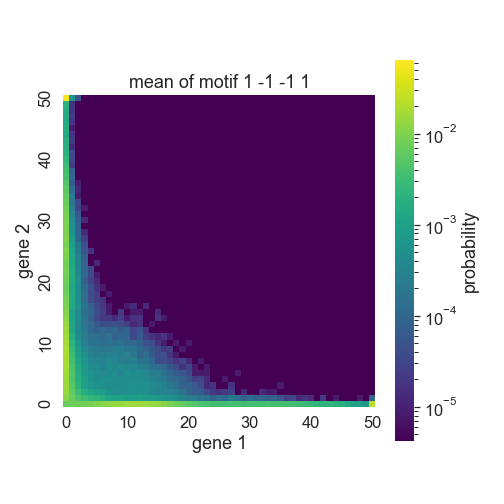
\includegraphics{../analysis/eda/first-set-heatmaps/summaries/57-mean.png}
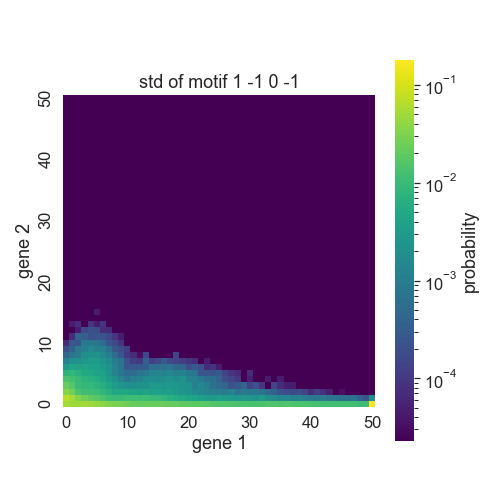
\includegraphics{../analysis/eda/first-set-heatmaps/summaries/57-std.png}

This one is mutual repression, self activation.

\hypertarget{methods}{%
\subsection{Methods}\label{methods}}

Provide a description of the technical/methodological approach that
chose for your project. State assumptions clearly.

We used several different machine learning methods for making
predictions: multinomial logistic regression (ML), random forest (RF),
and k nearest neighbors (KNN).

ML \ldots{}

RF uses an ensemble of decision trees. A decision tree splits the data
using binary questions that maximize information gain for that split in
the data. Once a tree is fit, prediction for a observation follow from
which branches it follow in the tree. Using a single tree tends to
result in over fitting and poor prediction on out of sample data. RF is
one of the methods used for dealing the short-comings of decision trees.
For RF, a individual tree is fitted to a sample, which has the same size
as the training data and is sampled with replacement, from the training
data. For each split in the tree, only a random selection of a specified
proportion of the features are considered. Many trees trained on randoms
samples using random selected features for each split are brought
together to make a `random forest'. When predicting with a RF, the
predicted category is whatever category was predicted most frequently by
the trees in the forest.

KNN is an algorithm that relies on the how close points are to each
other for prediction. It works like this: To predict the class for a new
point, find a specified number (k) of the closest points in euclidean
space to that point; use the most frequent class among those neighbors
to predict the class of the new point. As may be guess from the
description, a major draw back of KNN is that it does not perform well
when the outcomes are not clustered, such as when categories live each
others' neighborhood. (This might actually be a problem for all
prediction though) In our implementation of KNN, we scaled the features
using \texttt{standardscaler} from the SKLearn package to avoid giving
certain features more weight in the prediction.

An assumption for all of these methods is that the data use to train and
test them are representative. This assumption is not meet when
considering the empirical data since the simulated data does not have
sampling loss like the empirical does. Before doing prediction on
empirical data these methods would need to be train and tested on data
which adjusts for this, as well as other factors that may make the
simulated data non-representative of the empirical.

\hypertarget{results}{%
\subsection{Results}\label{results}}

Describe inferential and/or predictive results of your analysis. Try to
avoid showing large tables and use graphics if possible instead.

\hypertarget{discussion-and-conclusion}{%
\subsection{Discussion and Conclusion}\label{discussion-and-conclusion}}

Discuss what insights you gained from your project, in bullet form as
follows: - Provide summary of your findings - What are limitations of
your analyses? How can they be remedied in the future work?

\hypertarget{works-cited}{%
\subsection{Works Cited}\label{works-cited}}

Cao, J., Spielmann, M., Qiu, X. et al.~The single-cell transcriptional
landscape of mammalian organogenesis. Nature 566, 496--502 (2019).
\url{https://doi.org/10.1038/s41586-019-0969-x}

Gallivan CP, Ren H and Read EL (2020) Analysis of Single-Cell Gene Pair
Coexpression Landscapes by Stochastic Kinetic Modeling Reveals Gene-Pair
Interactions in Development. Front. Genet. 10:1387. doi:
10.3389/fgene.2019.01387

\end{document}
